\chapter{\rustsec{}: A SeKVM Rust Rewrite}
\label{sec:migration}

\section{Integration with Linux}

challenge: Linux 5.15 does not include Rust support

solution: our way of source code organization, build system integration,
how we link Rust and C, data layout issues, etc.

\section{Bringing up \rustsec{} on Real Hardware}

We chose the Raspberry Pi model 4B (Rpi-4B) to verify our implementation on
real hardware.
%This section describes the problem that occured when trying to run SeKVM on
%Rpi-4B, and how we solved the issue.
SeKVM's trusted core \secore{} originally reserved its private memory by
defining global symbols whose addresses reside right after the kernel image,
in the Linux kernel linker script.
\secore{} then references those symbols to access and utilize the reserved
memory.
However, there exists an unusable hole in Rpi-4B's physical memory address
space, and the bootloader of Rpi-4B places the kernel image before the hole,
resulting in an overlap of \secore{}'s private memory and the unusable hole
(\autoref{fig:overlap}). This makes SeKVM unable to initialize on Rpi-4B.

\begin{figure}[hbtp]
    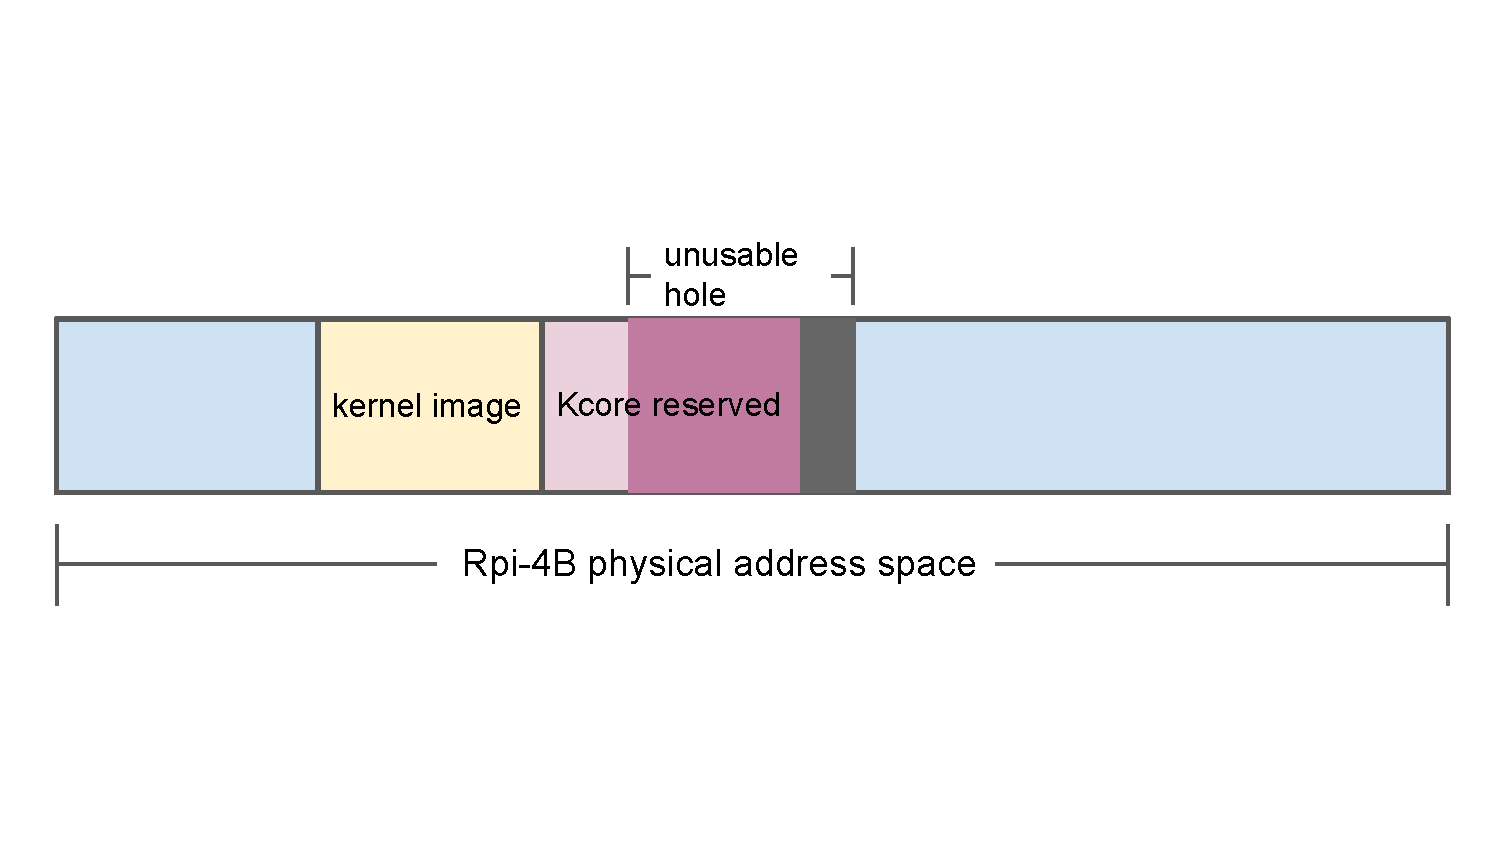
\includegraphics[scale=0.60]{figures/overlap.pdf}
    \caption{Kcore overlaps the unusable hole on Rpi-4B}
    \label{fig:overlap}
\end{figure}

To solve this issue, instead of allocating memory in the linker script,
we first locate a range of memory which does not overlap with the unusable hole
of Rpi-4B and the kernel image, then call \code{memblock\_reserve} to
mark the range of memory as reserved so that the kernel does not accidentally
access this memory range (\autoref{fig:rcorereserved}).
The global symbols have also been changed to C macros that expand into
addresses in the reserved range for \rustsec{}'s \rustcore{} usage.

\begin{figure}[H]
    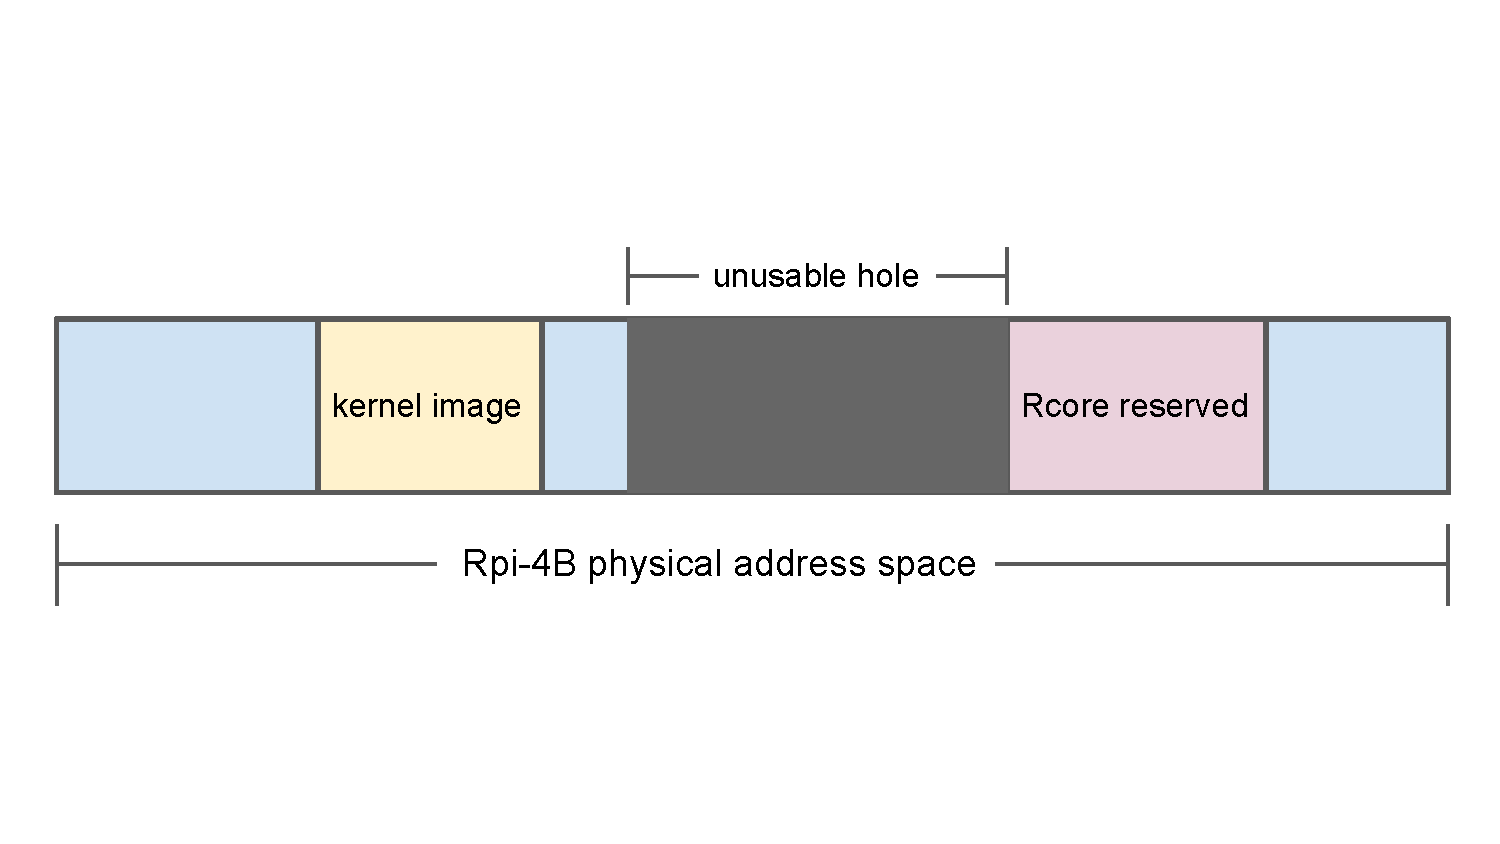
\includegraphics[scale=0.60]{figures/rcore_reserved.pdf}
    \caption{Overlap prevention}
    \label{fig:rcorereserved}
\end{figure}

\section{Code Migration}

challenge: difficult to do a top-down design due to the difficulty to debug
and complexity of a hypervisor (is this challenge kinda weak?)

solution: two pass method, first function-by-function rewrite, then remove
unsafe and redesign after we have a working Rust hypervisor, and leverage
Rust to achieve a stronger memory region isolation guarantee.

